\ifmostrarGabarito
\textbf{Resposta: (D)}

\textbf{Justificativa:}
A classe filha \texttt{SensorSonar} herda de \texttt{Sensor}.
1. No construtor \texttt{\_\_init\_\_}, \texttt{super().\_\_init\_\_(identificador)} inicializa o atributo herdado \texttt{self.id = "SN-01"}.
2. No método \texttt{obter\_status}, a chamada \texttt{super().obter\_status()} executa a versão da classe base, retornando \texttt{"Sensor SN-01: ATIVO"}.
3. O método concatena \texttt{" (Prof: 300.0m)"}, gerando a string completa: \texttt{"Sensor SN-01: ATIVO (Prof: 300.0m)"}.
\else
\par\vspace{0.15cm}
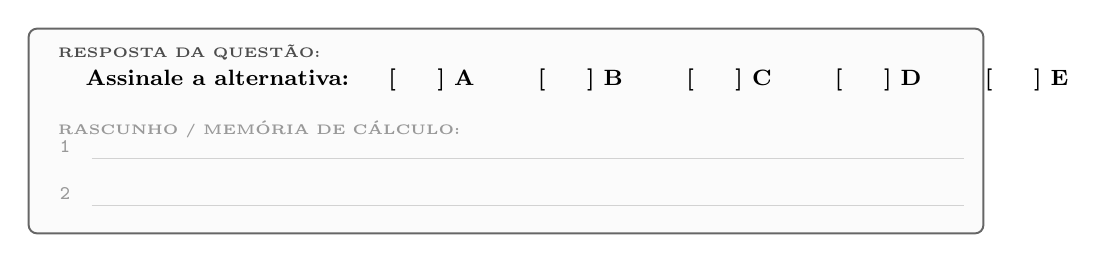
\begin{tikzpicture}
  \draw[rounded corners=3pt, draw=black!60, line width=0.7pt, fill=gray!3] (0,0) rectangle (\linewidth, -2.6cm);
  \node[anchor=north west, font=\tiny\bfseries\color{black!70}] at (0.25cm, -0.08cm) {RESPOSTA DA QUESTÃO:};
  \node[anchor=west, font=\footnotesize\bfseries] at (0.6cm, -0.65cm) {Assinale a alternativa: \quad [ \hspace{0.3cm} ] A \qquad [ \hspace{0.3cm} ] B \qquad [ \hspace{0.3cm} ] C \qquad [ \hspace{0.3cm} ] D \qquad [ \hspace{0.3cm} ] E};
  \node[anchor=north west, font=\tiny\bfseries\color{gray!80}] at (0.25cm, -1.05cm) {RASCUNHO / MEMÓRIA DE CÁLCULO:};
  \draw[gray!35, line width=0.4pt] (0.8cm, -1.65cm) -- (\linewidth-0.25cm, -1.65cm);
  \draw[gray!35, line width=0.4pt] (0.8cm, -2.25cm) -- (\linewidth-0.25cm, -2.25cm);
  \node[anchor=east, font=\scriptsize\ttfamily\color{gray!80}] at (0.65cm, -1.5cm) {1};
  \node[anchor=east, font=\scriptsize\ttfamily\color{gray!80}] at (0.65cm, -2.1cm) {2};
\end{tikzpicture}
\par\vspace{0.2cm}
\fi
